\documentclass[12pt]{article}

% pacotes utilizados
\usepackage{cancel}
\usepackage{graphicx} 
\usepackage{amssymb}
\usepackage[portuguese]{babel}
\usepackage[a4paper,top=3cm,bottom=2cm,left=3cm,right=2cm]{geometry}
\usepackage{ascii}
\usepackage{amsmath}
\usepackage{amssymb}
\usepackage{amsfonts} 
\usepackage{tikz}
\usepackage[utf8]{inputenc}
\usepackage{listings}
\usepackage{parskip}
\usepackage{enumitem}
\usepackage{float}


\linespread{1.5}
\title{Aula do dia 14 de dezembro de 2023}
\author{
    \begin{tabular}{rl}
        Autor: & Rodrigo Bissacot Proença \\
        Transcrito para \LaTeX por: & Lucas Amaral Taylor
    \end{tabular}
}
\date{\today}

\begin{document}
    \maketitle
    \section*{Definição}
    Temos que $X \subseteq \mathbb{R}$ e $f: X \to \mathbb{R}$ uma função injetora, dizemos que $f$ é \textbf{homeomorfismo sobre a imagem quando}:
    \begin{equation*}
        g: f(x) = Y \to \mathbb{R} \text{ é contínua}
    \end{equation*}
    \begin{equation*}
        y = f(x) \mapsto g(y) = x
    \end{equation*}

    \textit{Observação: } $x$ é único, pois $f$ é injetora.

    \textit{Notação: para } $g=f^-1$.

    \subsection*{Exemplo de função contínua injetora com inversa descontínua}
    \begin{equation*}
        f: \left[ 0, 1 \right) \cup \left[2, 3\right] \to \mathbb{R}
    \end{equation*}
    \begin{equation*}
        f(x)= 
        \begin{cases}x, & \text{se}  0\leq x<1 \\ 
        x-1, & \text{ se } \quad 2 \leq x \leq 3
        \end{cases}
    \end{equation*}

    é contínua e é \textbf{injetora}
    \begin{figure}[H]
        \centering
        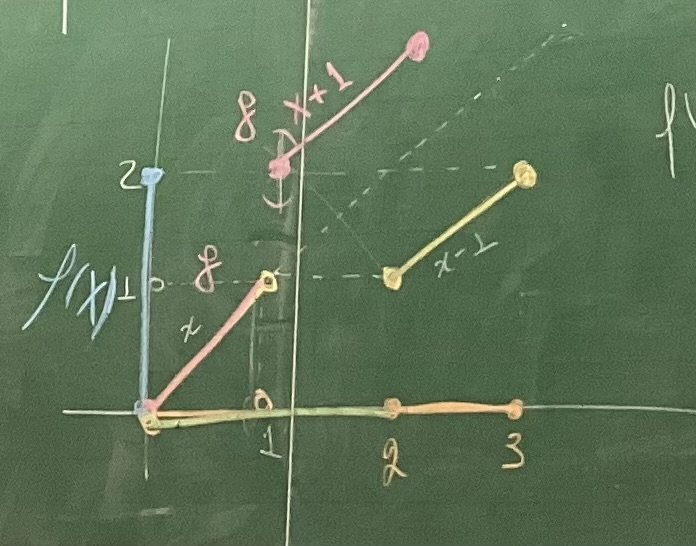
\includegraphics[scale = 0.5]{IMG_1438.jpeg}
        \caption{Gráfico das funções}
        \label{fig:graf}
    \end{figure}
    Note que o conjunto imagem de $f$ é dado por:
    \begin{equation*}
        \text{Im} f = f(X) = f\left(\left[0,1\right] \cup \left[2, 3\right]\right) = \left[0,2\right]
    \end{equation*}
    \begin{equation*}
        f^-1 = g:\left[0, 2\right] \to X = \left[0,1\right) \cup \left[2,3\right]
    \end{equation*}
    \begin{equation*}
        g(x)= 
        \begin{cases}
        x, & \text{ se } 0 \leq x <1 \\
        x-1, & \text{ se }\quad 2 \leq x \leq 3
        \end{cases}
    \end{equation*}

    \textbf{Exercício} Mostre que $g$ é descontínua em 1. \textbf{Dica:} $\varepsilon = \frac{1}{2}$. 

    \textit{Observações:}
    \begin{enumerate}
        \item Outra maneira de ver que $g$ não é contínua é que $g\left(\left[ 0,2 \right]\right) = \left[0,1\right)\cup\left[2,3\right]$
        \textbf{Ou seja, $g$ não leva intervalo em intervalo}

        \item Note que o domínio de $X$ de $f$ \textbf{não é compacto} e não é um intervalo.
    \end{enumerate}

    \section*{Funções contínuas em compactos}
    \subsection*{Proposição}
     Seja $K \subseteq \mathbb{R}$ \textbf{compacto}. Se $f: K \to \mathbb{R}$ contínua, então $f(K)$ é compacto. 
     
     \textbf{Observação: Vale para espaços métricos}

    \subsection*{Prova}
     Usaremos a caracterização de compactidade vida sequências. 
     
     Seja $(y_n)_n$ uma sequência em $f(K)$.
     
     \textbf{A mostrar: } existe $(y_n)_n$ tal que $\lim \limits_{K \to + \infty} y_{n_k} = y \in f(K)$

    \begin{equation*}
        y_n \in f(K) \forall n \in \mathbb{N}
    \end{equation*}

    Isso implica que:
    \begin{equation*}
        \exists x_n \in K \text{ tal que } f(x_n) = y_n \text{ , } \forall n \in \mathbb{N}
    \end{equation*}
    \begin{equation*}
        \implies (x_n)_n \text{ é uma sequência em } K
    \end{equation*}

    Como $K$ é compacto, temos que $\exists (x_{n_k})_k$ uma subsequência de $(x_n)_n$ tal que $\lim \limits_{K \to + \infty} x_{n_k} = x \in K$.

    Como $f$ é contínua, segue que:
    \begin{equation*}
        \lim \limits_{k \to \infty} f(x_{n_k}) = f(x) \in f(K)
    \end{equation*}

    \textbf{Provamos que: } Dada uma sequência em $f(k)$, existe uma subsequência $(y_{n_k})_k$ tal que:
    \begin{equation*}
        \lim \limits_{k \to \infty} y_{n_k} = \lim \limits_{k \to \infty} f(x_{n_k}) = f(x) \in f(K)
    \end{equation*}

    Logo, $f(K)$ é compacto.

    \subsection*{Corolário (usado na lista 03)}
    Se $K$ é um compacto e $f: K \to \mathbb{R}$ é contínua entáo $f$ assume máximo e mínimo em $K$. Ou seja, existem $x_0$ e $x_1$ em $K$ tais que:
    \begin{equation*}
        f(x_0) \leq f(x) \leq f(x_1) \text{ , } \forall x \in K
    \end{equation*}

    \textbf{Prova}

    $K$ é compacto e $f: K \to \mathbb{R}$ contínua implica $f(K)$ é compacto. Se $f(K)$ é compacto, então $f(K)$ é fechado e limitado. Se $f(K)$ é limitado, então existem $\inf f(K)$ e  $\sup f(K) \in \mathbb{R}$. 

    \textbf{A mostrar: } $y_1 = \sup f(K) \in f(K)$
    \begin{equation*}
        \forall n \in \mathbb{N} \text{ , } \exists x_0 \in K \text{ tal que } y_1 - \frac{1}{n} < f(x_n) < y_1
    \end{equation*}
    \begin{equation*}
        \implies \lim \limits_{n \to \infty} f(x_n) = y_1 \implies y_1 \in \overline{f(K)} = f(K)
    \end{equation*}
    
    \textit{Observação: } $f(K)$ é fechado

    \begin{equation*}
        y_1 = \sup f(K) \in f(K) \implies \exists x_1 \in K \text{ tal que } f(x_1) = y_1
    \end{equation*}

    \textbf{Exercício: } Mostrar que:
    \begin{equation*}
        \inf f(K) = \min f(K) = f(x_0) \text{ para algum } x_0 \in K
    \end{equation*}

    \subsection*{Corolário}
    Seja $f: \left[a,b\right] \to \mathbb{R}$ com $f$ contínua. Então:
    \begin{equation*}
        f(\left[a, b\right] = \left[c, d\right] = \left[f(x_0), f(x_1)\right]
    \end{equation*}

    \textbf{Função contínua leva intervalos fechados e limitados em intervalos fechados e limitados}
    
    \textit{Lembre-se que \textbf{Intervalo fechado e limitado} é \textbf{compacto}}

    \subsubsection*{Exemplo}
    \begin{equation*}
        f: \left[ a, + \infty \right) \to \mathbb{R}
    \end{equation*}
    \begin{equation*}
        x \mapsto f(x) = \frac{1}{x}
    \end{equation*}
    \begin{equation*}
        f\left( \left[a, + \infty \right) \right) = \left( 0, \frac{1}{a}\right]
    \end{equation*}

    \textbf{Mas não é verdade que funções contínuas levam intervalos fechados em intervalos fechados}

    \section*{Teorema}
    $k \subseteq \mathbb{R}$ é compacto então $f: K to \mathbb{R}$ é contínua  e injetora é \textbf{homeo} sobre a imagem.

    Ou seja, 
    \begin{equation*}
        g = f^{-1} \cdot f(K) \to K
    \end{equation*}
    \begin{equation*}
        y = f(x) \mapsto g(y) = x
    \end{equation*}

    é contínua.

    \textbf{Prova: } Usando a caracterização de continuidade via sequências:

    Dado $y \in f(K)$, queremos mostrar que $g$ é contínua em $y$. 
    \begin{equation*}
        y \in f(K) \iff \exists x_0 \in K \text{ tal que } f(x_0) = y_0
    \end{equation*}

    Devemos mostrar que, para qualquer $(y_n)_n$ em $f(K)$ tal que $\lim \limits_{n \to \infty} y_n = y_0$, temos que:
    \begin{equation*}
        \lim \limits_{n \to \infty} g(y_n) = g(y_0)
    \end{equation*}

    Uma maneira de mostrar que $\lim \limits_{n \to \infty} g(y_n) = g(y_0)$ é mostrar que toda subsequência convergente $\left(g(y_{n_k}) \right)_{k \in \mathbb{N}}$ para $g(y_0)$. Isso implica que a sequência de $\left( g(y_n)\right)_{n \in \mathbb{N}}$ tem um \textbf{único valor de aderência}.

    \begin{equation*}
        \implies \liminf \limits_{n \to \infty} \inf g(y_n) = \limsup \limits_{n \to \infty} g(y_n) = g(y_0)
    \end{equation*}
    \begin{equation*}
        \exists \lim \limits_{n \to \infty} g(y_n) = g(y_0)
    \end{equation*}

    \textit{Note que }$g: f(K) \to K$. Portanto, qualquer sequência $g\left(g(y_n)\right)_n$ em $K$ é limitada. Logo, $\left(g(y_n)\right)_\mathbb{N}$ possui uma subsequência que converge.
\end{document}